\documentclass{article}
\usepackage{graphicx}
\graphicspath{ {C:/Users/Finlay/Documents/Projects/project2/figs/} }
\usepackage{amsmath}
\usepackage[margin=1in]{geometry}
\usepackage{float}

\begin{document}

\title{Using Contact Tracing Data to inform inference of transmission networks}
\author{Finlay Campbell}

\maketitle

\section{Introduction}
	\begin{itemize}
		\item The value and importance of outbreak reconstruction
		\item The problems and issues with outbreak reconstruction
		\begin{itemize}
			\item Integrating multiple data sources in non-arbitrary ways
			\item Existing data sources having an insufficient information content
		\end{itemize}
		\item Describe various previous approaches to outbreak reconstruction, with their respective benefits and drawbacks
		\item Introduce Outbreaker as an integrated Bayesian approach
		\begin{itemize}
				\item Describe general approach of Outbreaker
				\item Describe situations in which Outbreaker struggles (mutation rate too low, generation time too broad, etc.)
				\item CTD as an additional data source is able to fill many of these gaps 
		\end{itemize}	
		\item Describe the availability and types of CTD available, and the benefit of CTD over other types of genetic and epidemiological data
		\item Describe previous uses of CTD in informing outbreak reconstruction
		\item Describe the aim of this project: integrating CTD as an additional data source to inform outbreak reconstruction in a Bayesian framework
	\end{itemize}

\section{Methods}
\subsection{Simulating CTD}
	CTD is simulated from known transmission networks and used to test the potential of CTD in informing outbreak reconstruction. Our simulation function incorporates the probability of observing contact between a transmission pair ($\epsilon$) in order to simulate CTD of variable coverage and sensitivity, as well as a scaling factor ($\xi$) to describe the probability observing contact between individuals not in a transmission pair, relative to $\epsilon$. This allows the simulation of misinformative CTD. The probability of observing contact ($c_{ij}$=TRUE) between any two individuals is calculated as follows:
	
	\begin{gather}
	\text{For transission pairs | } p(c_{ij}=\text{TRUE}) = \epsilon \\
	\text{For non-transission pairs | } p(c_{ij}=\text{TRUE}) = \epsilon*\xi
	\end{gather}

\subsection{Contact Tracing Likelihood}
	The contact tracing likelihood $\Omega_3$ describes the probability of obtaining the observed contact relationship between two individuals ($c_{ij}$=TRUE or FALSE), given the proposed transmission network. It uses a contact reporting probability $\epsilon$ as its only parameter, describing the probability of observing contact ($c_{ij}$=TRUE) between a transmission pair. The probability of not observing contact ($c_{ij}$=FALSE) is therefore the compliment of $\epsilon$. Formally, the contact tracing likelihood is described as follows:
	
	\begin{gather}
	\text{For $c_{ij}$ = TRUE | } \Omega_3 = \epsilon \\
	\text{For $c_{ij}$ = FALSE | } \Omega_3 = 1-\epsilon
	\end{gather}

	\section{Results}

	\begin{figure}[H]
		\centering
		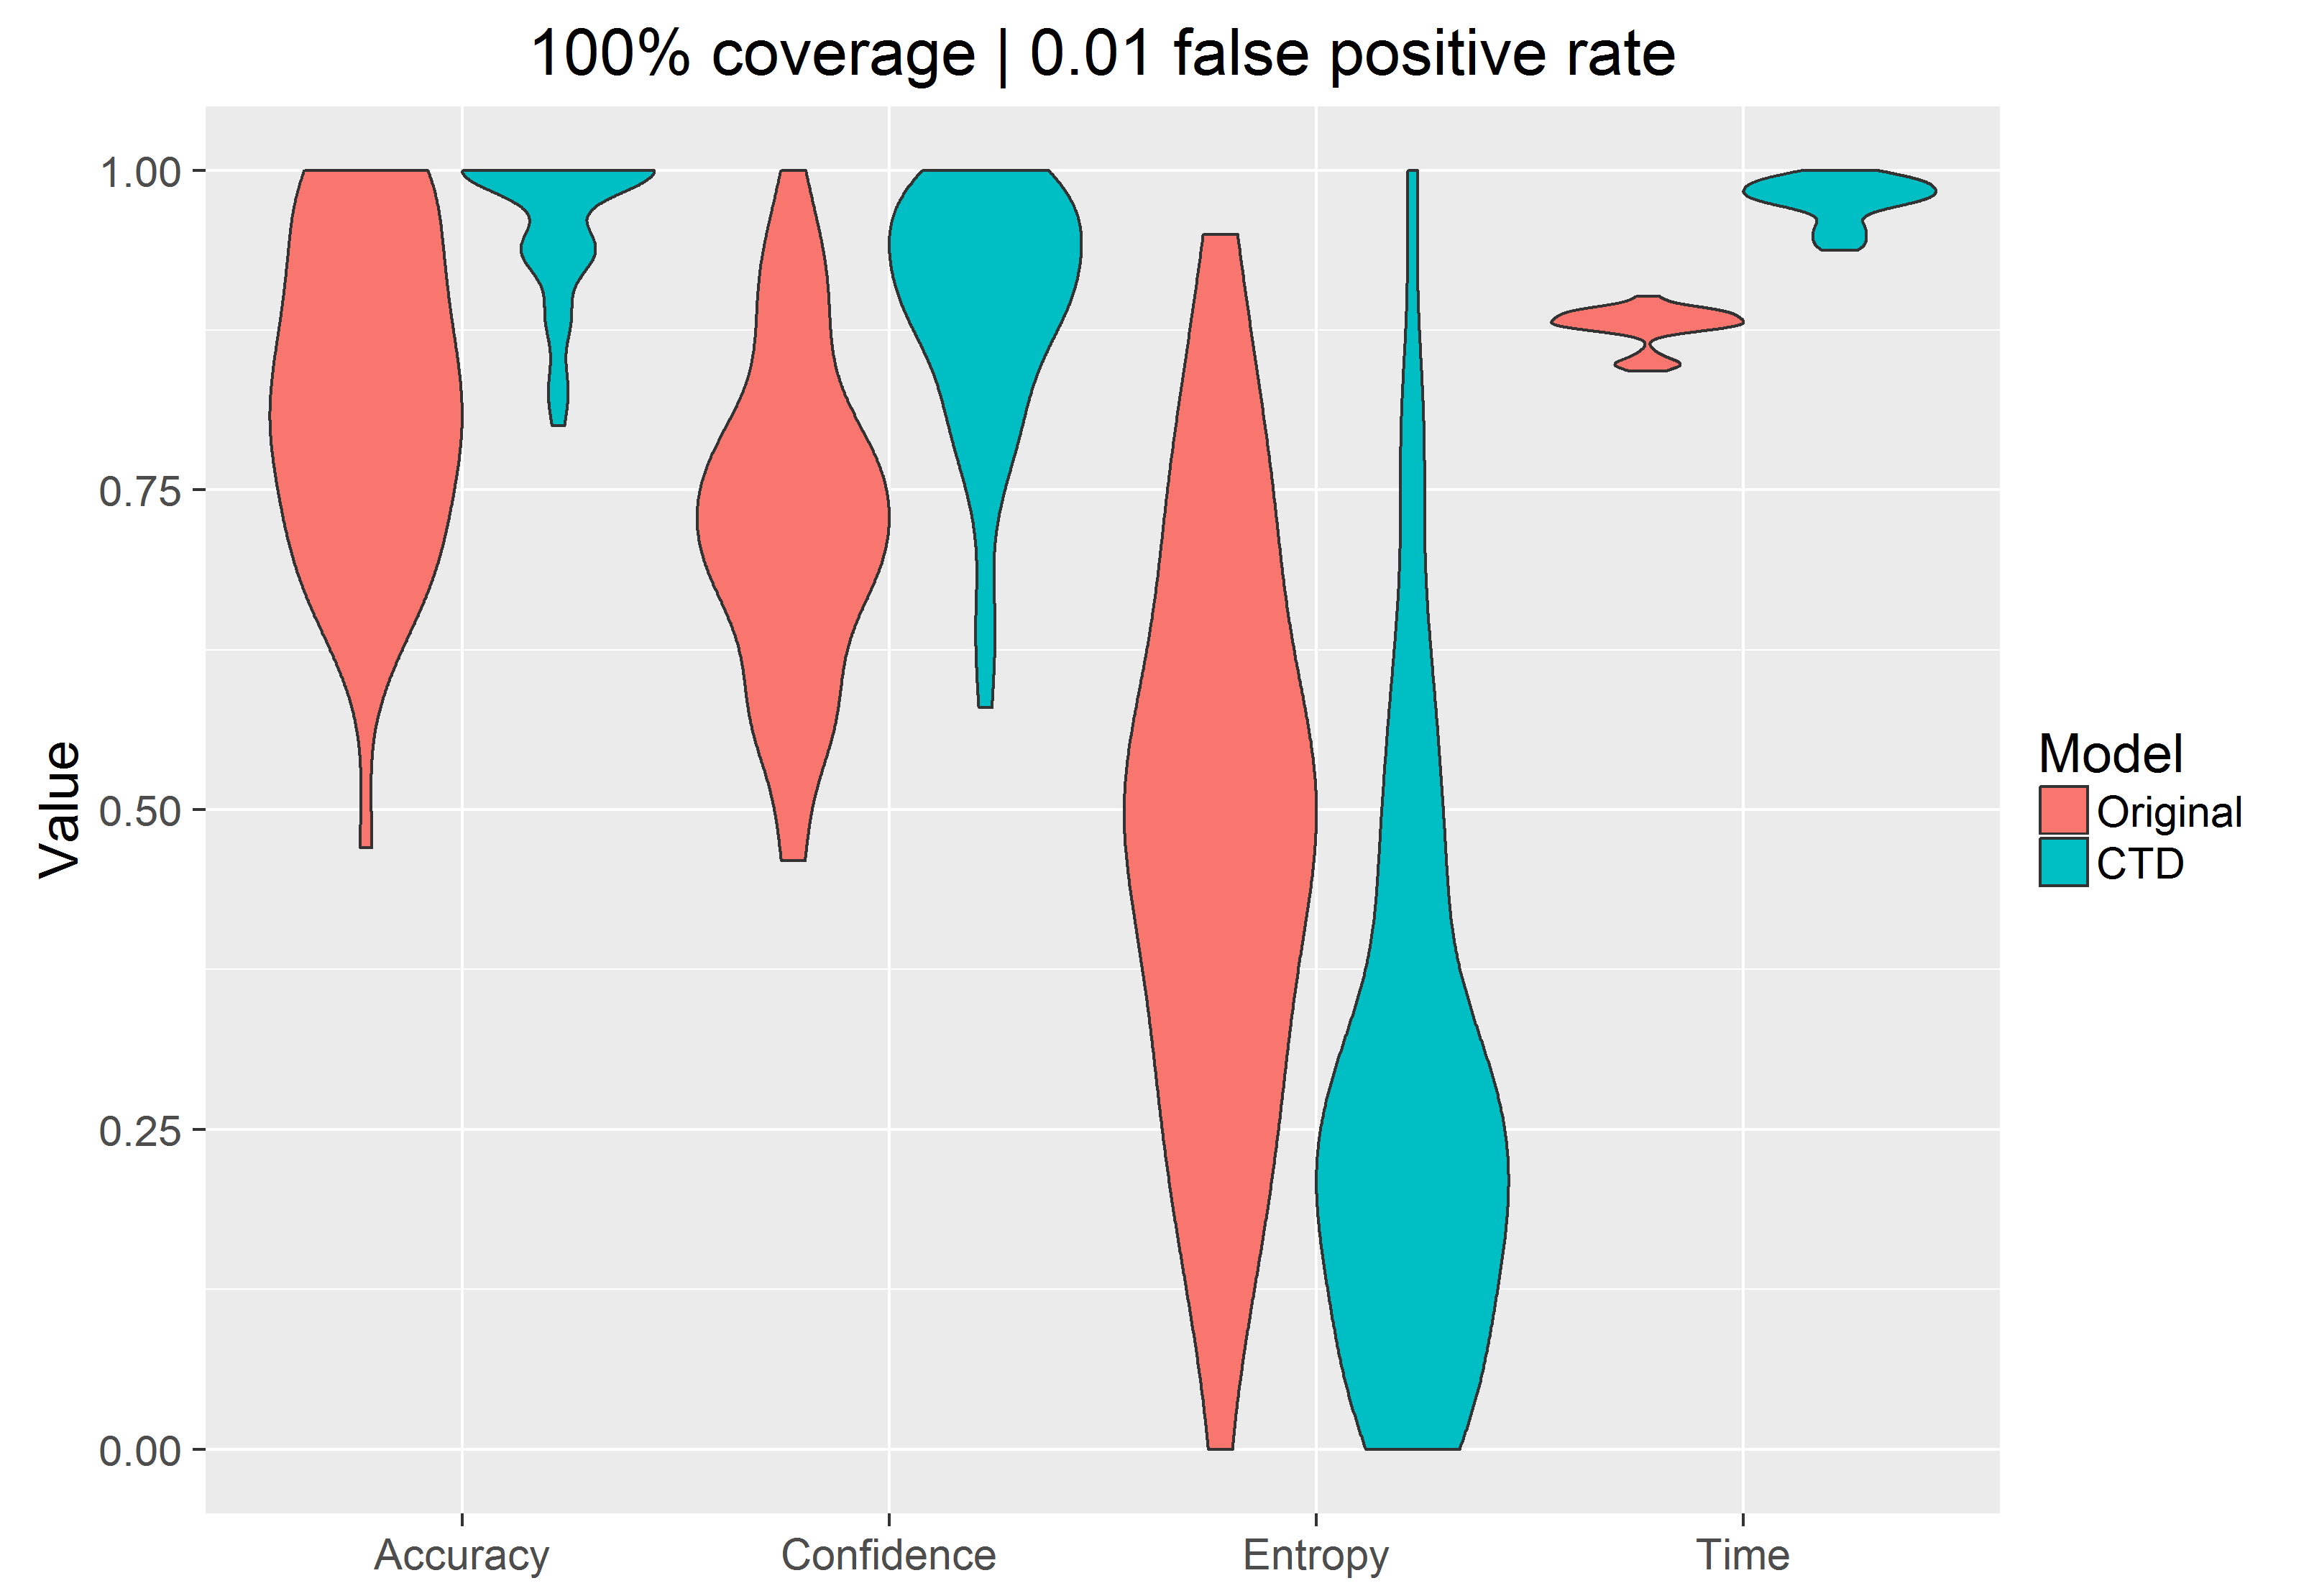
\includegraphics[width=5.0in]{eps010xi001.png}
		\caption{Performance changes upon incorporating contact tracing data into Outbreaker2 ($\epsilon$=1, $\xi$=0.01)}
	\end{figure}
	
	\begin{figure}[H]
		\centering
		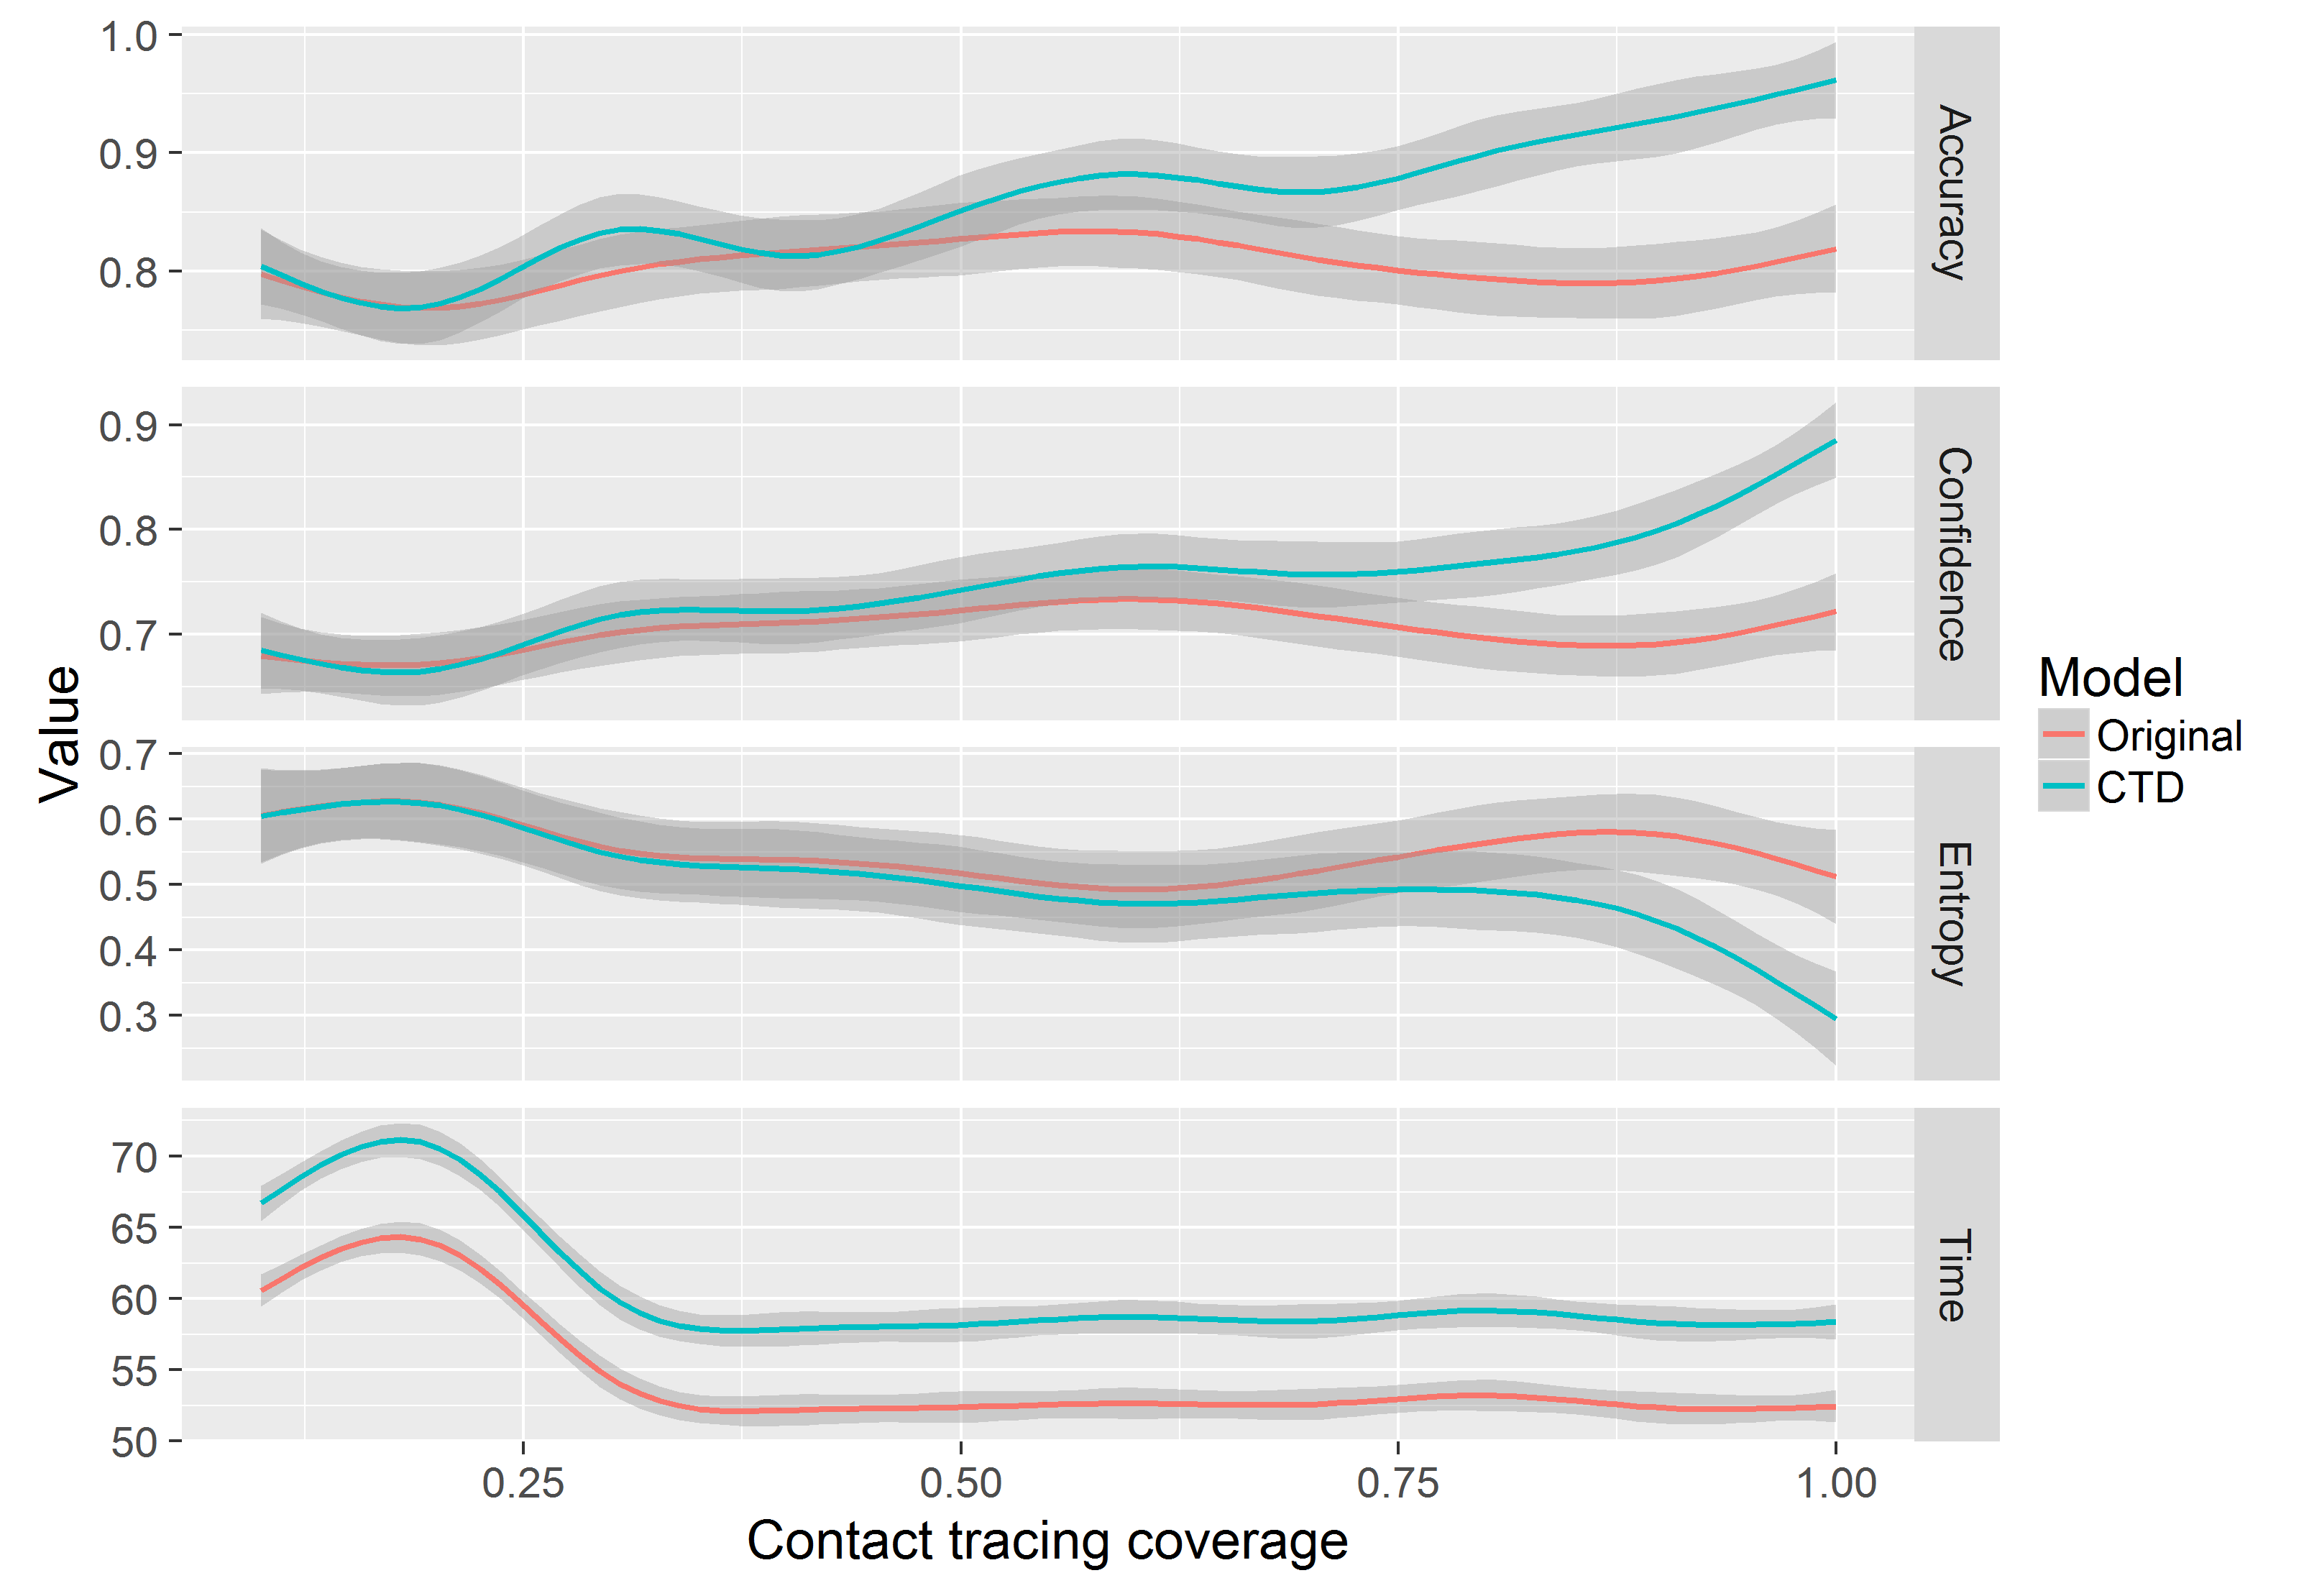
\includegraphics[width=5.0in]{smoothanalysis.png}
		\caption{Relative performance changes of CTD.outbreaker with contact tracing coverage of simulated CTD}
	\end{figure}
		
	\begin{figure}[H]
		\centering
		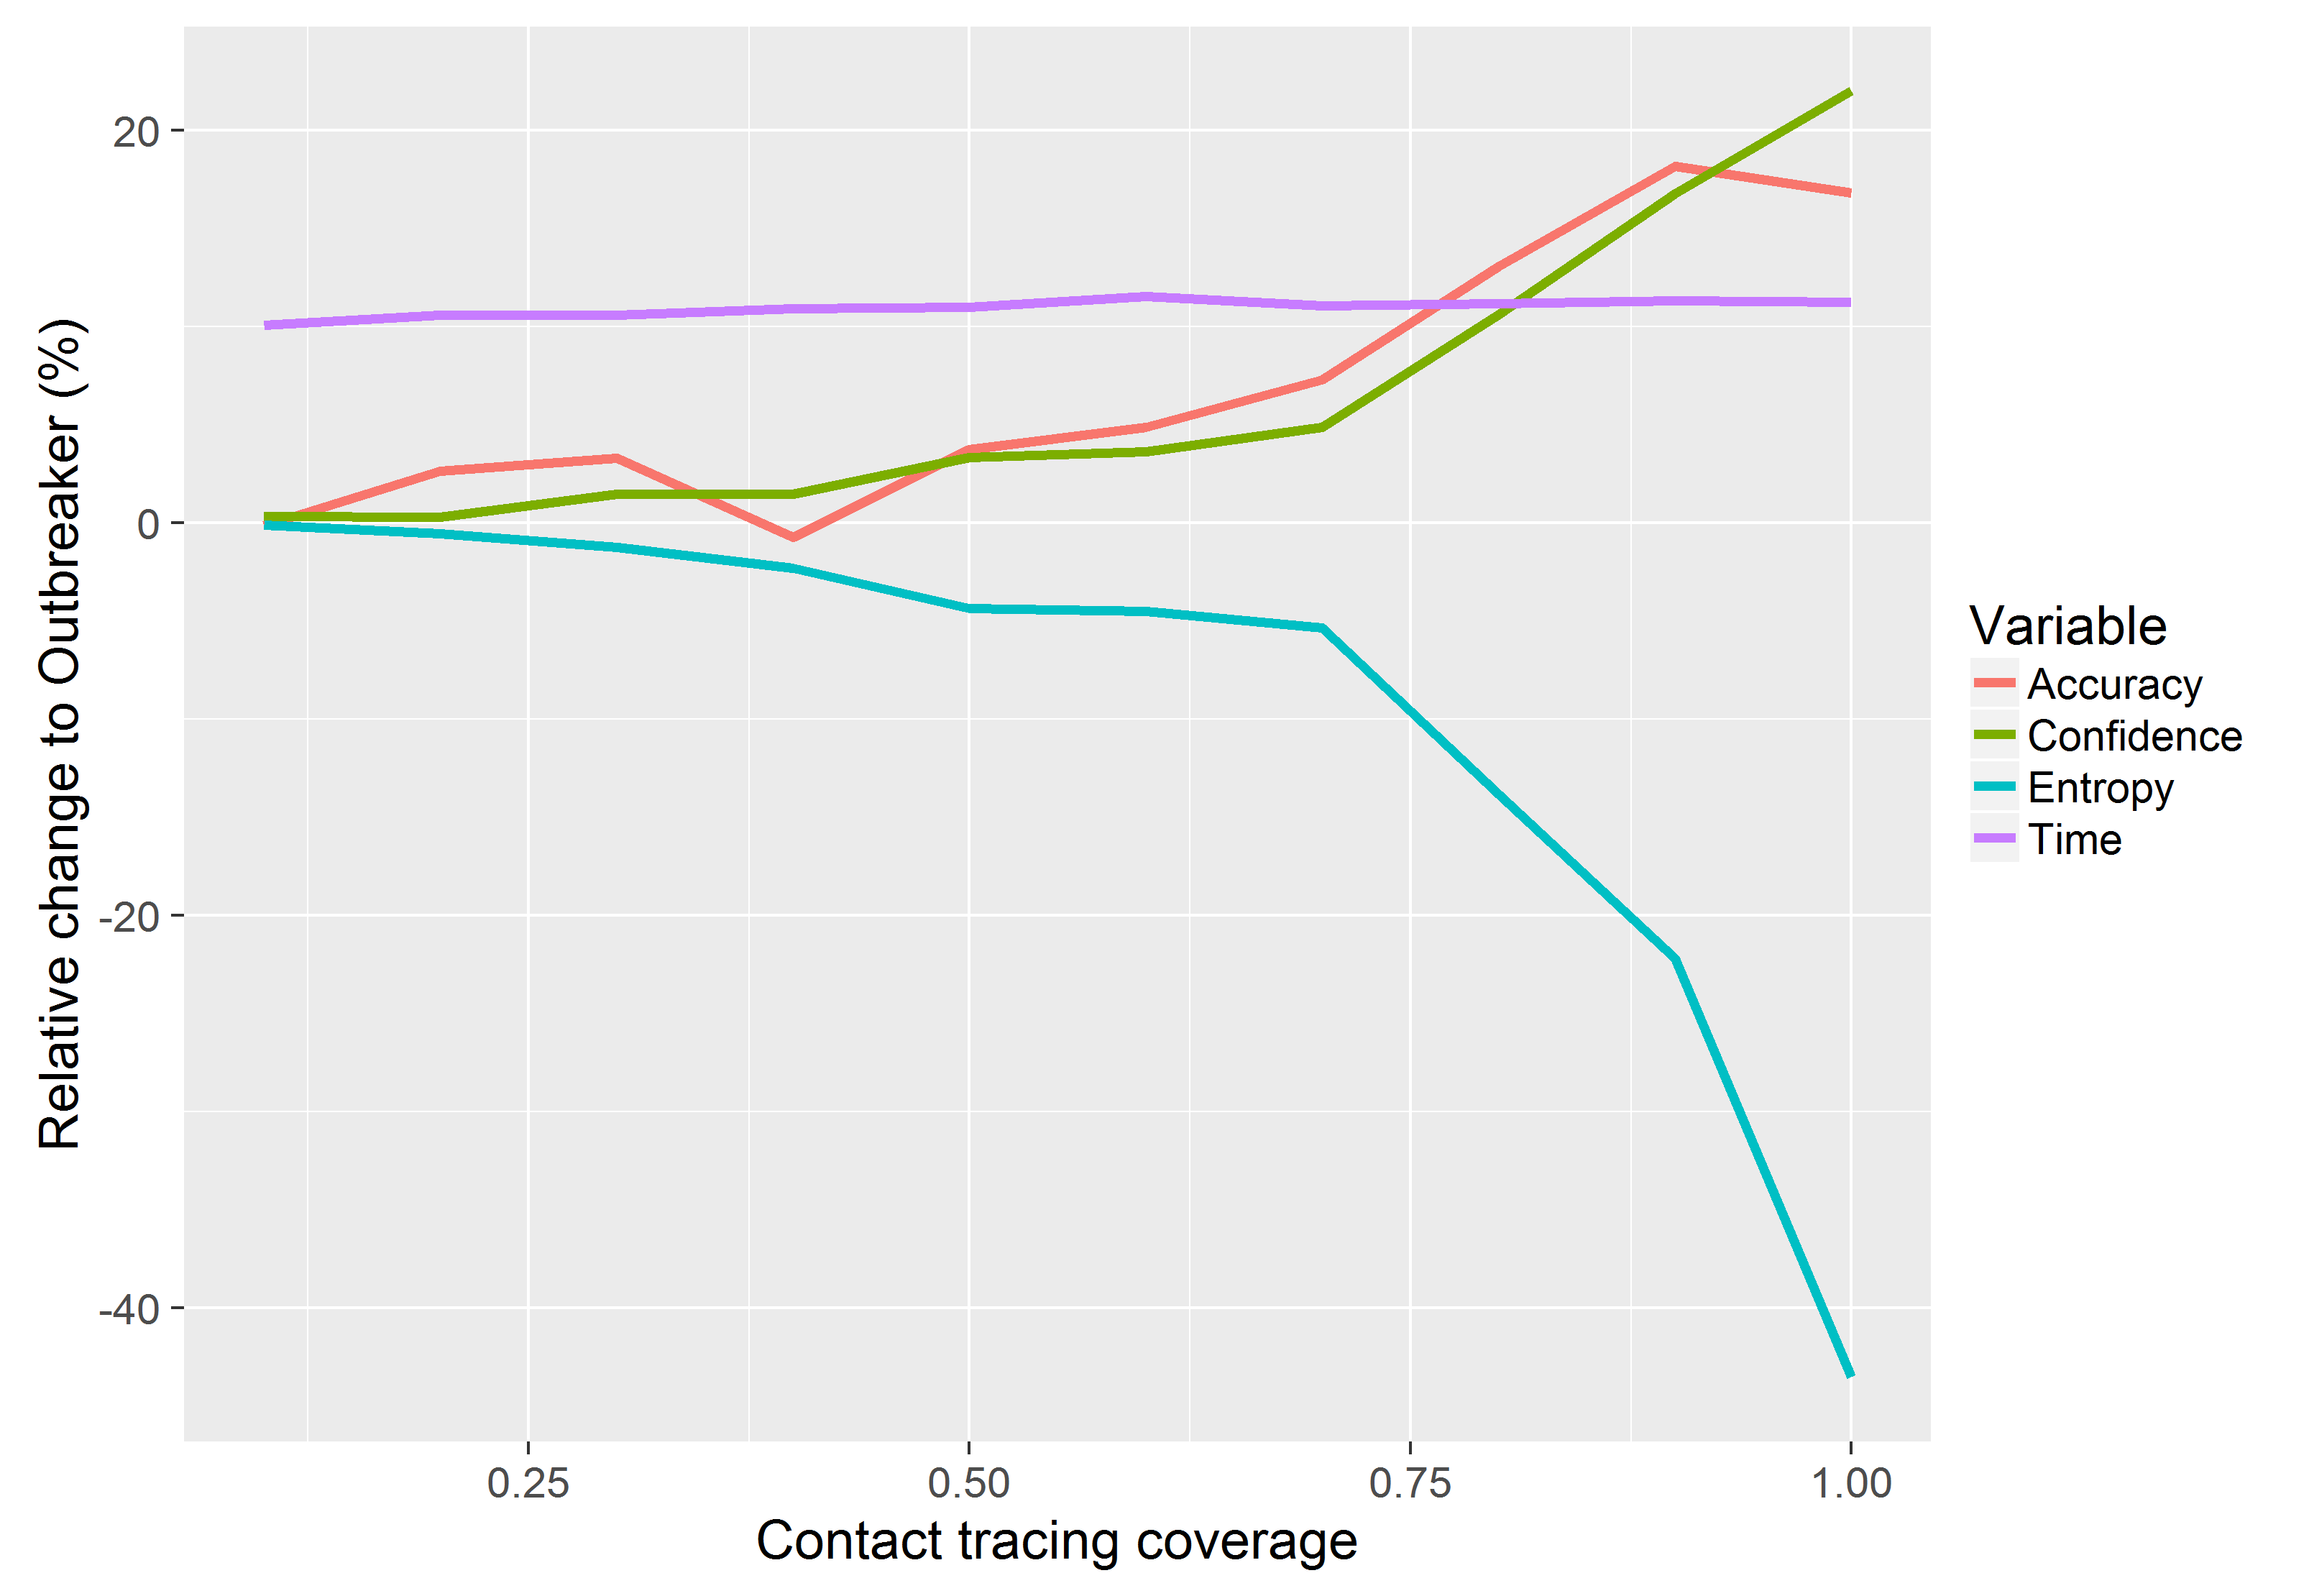
\includegraphics[width=5.0in]{relativeanalysis.png}
		\caption{Performance changes of CTD.outbreaker with contact tracing coverage of simulated CTD}
	\end{figure}	
	
	\section{To do:}
		
	\begin{itemize}
		\item Do a grid of xi/eps
		\item Make table of things to look at and then decide
		\item Look at large/small outbreak
		\item Look at high/low mutation
		\item SimOutbreak allows superspreading (0.1 of superspreader R0 or 5 times higher)
		\item Value for R0/generation time
		\begin{itemize}
			\item Use Ebola values
			\item Or SARS (but strong genetic signature)
			\item But also look at high/low R0 (might make it more difficult)
			\item Central setup being similar to Ebola
			\item Then do theoretical examples for other situations
		\end{itemize}
		\item Add prior for eps in description
		\item (DONE) Label order for relative.performance
		\item (DONE) Don't enforce scaling on violinplot
		\item (DONE) Add uncertainty to absolute.plot
		
	\end{itemize}
	
	
\end{document}
